\documentclass[12pt]{article}
\usepackage{amsfonts, amssymb, amsmath, amsthm}
\usepackage[margin=1in]{geometry}
\usepackage{tikz}
\usetikzlibrary{patterns, decorations.pathreplacing}

\pagestyle{myheadings}
\markright{Explainer: Rudin 4.24 --- Midpoint Convexity Implies Convexity\hfill}

\newcommand{\R}{\mathbb{R}}

\begin{document}

\begin{center}
    \textbf{\Large Midpoint Convexity Implies Convexity}\\[0.5em]
    \large A visual guide to Rudin 4.24
\end{center}

\section{Convexity vs Midpoint Convexity}

\begin{center}
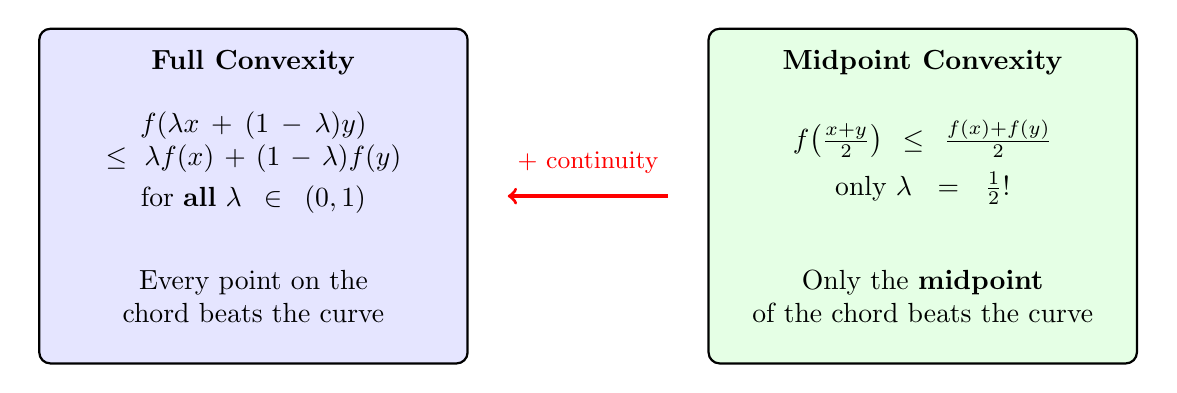
\begin{tikzpicture}[scale=0.85]
    % Full convexity
    \begin{scope}[xshift=-5cm]
        \draw[thick, rounded corners, fill=blue!10] (-3.2, -2.5) rectangle (3.2, 2.5);
        \node at (0, 2) {\textbf{Full Convexity}};
        \node[text width=5.5cm, align=center] at (0, 0.5) {
            $f(\lambda x + (1 - \lambda)y)$\\
            $\leq \lambda f(x) + (1 - \lambda) f(y)$\\[0.3em]
            for \textbf{all} $\lambda \in (0, 1)$
        };
        \node[text width=5cm, align=center] at (0, -1.5) {Every point on the\\chord beats the curve};
    \end{scope}

    % Midpoint convexity
    \begin{scope}[xshift=5cm]
        \draw[thick, rounded corners, fill=green!10] (-3.2, -2.5) rectangle (3.2, 2.5);
        \node at (0, 2) {\textbf{Midpoint Convexity}};
        \node[text width=5.5cm, align=center] at (0, 0.5) {
            $f\!\left(\frac{x + y}{2}\right) \leq \frac{f(x) + f(y)}{2}$\\[0.5em]
            only $\lambda = \frac{1}{2}$!
        };
        \node[text width=5cm, align=center] at (0, -1.5) {Only the \textbf{midpoint}\\of the chord beats the curve};
    \end{scope}

    % Implication arrow
    \draw[<-, very thick, red] (-1.2, 0) -- (1.2, 0);
    \node[red] at (0, 0.5) {\small + continuity};
\end{tikzpicture}
\end{center}

\section{Midpoint Convexity: The Picture}

\begin{center}
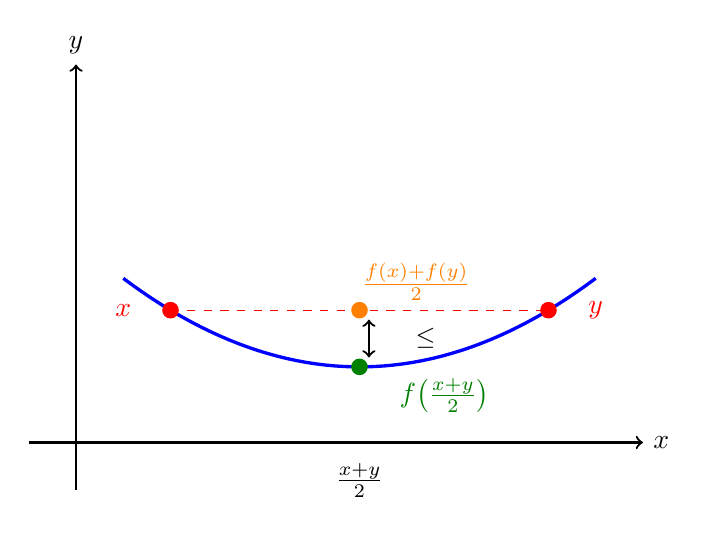
\begin{tikzpicture}[scale=1.2]
    \draw[thick, ->] (-0.5, 0) -- (6, 0) node[right] {$x$};
    \draw[thick, ->] (0, -0.5) -- (0, 4) node[above] {$y$};

    % Convex curve
    \draw[blue, very thick, domain=0.5:5.5, samples=50] plot (\x, {0.15*(\x - 3)*(\x - 3) + 0.8});

    % Two points
    \fill[red] (1, {0.15*4 + 0.8}) circle (2.5pt);
    \fill[red] (5, {0.15*4 + 0.8}) circle (2.5pt);
    \node[red] at (0.5, 1.4) {$x$};
    \node[red] at (5.5, 1.4) {$y$};

    % Chord
    \draw[red, dashed] (1, 1.4) -- (5, 1.4);

    % Midpoint on chord
    \fill[orange] (3, 1.4) circle (2.5pt);
    \node[orange] at (3.6, 1.7) {$\frac{f(x)+f(y)}{2}$};

    % Midpoint on curve
    \fill[green!50!black] (3, 0.8) circle (2.5pt);
    \node[green!50!black] at (3.9, 0.5) {$f\!\left(\frac{x+y}{2}\right)$};

    % Arrow
    \draw[<->, thick] (3.1, 0.9) -- (3.1, 1.3);
    \node at (3.7, 1.1) {\small $\leq$};

    \node at (3, -0.4) {$\frac{x+y}{2}$};
\end{tikzpicture}
\end{center}

\section{The Strategy: Bootstrap from $\lambda = 1/2$ to All $\lambda$}

\subsection{Step 1: Dyadic Rationals}

From $\lambda = 1/2$, we can get $\lambda = 1/4, 3/4$ by applying midpoints again:

\begin{center}
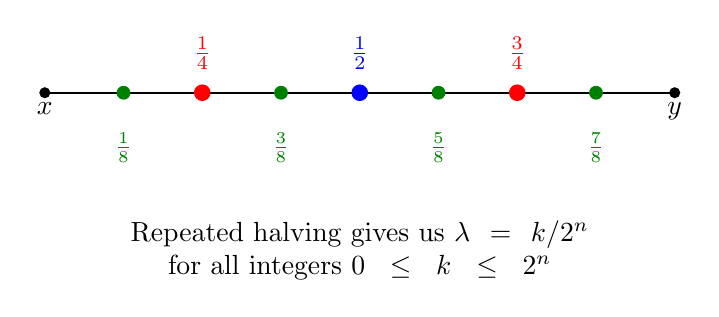
\begin{tikzpicture}[scale=1]
    % Number line from x to y
    \draw[thick] (0, 0) -- (8, 0);
    \fill (0, 0) circle (2pt) node[below] {$x$};
    \fill (8, 0) circle (2pt) node[below] {$y$};

    % Level 1: midpoint
    \fill[blue] (4, 0) circle (3pt);
    \node[blue] at (4, 0.5) {$\frac{1}{2}$};

    % Level 2: quarter points
    \fill[red] (2, 0) circle (3pt);
    \fill[red] (6, 0) circle (3pt);
    \node[red] at (2, 0.5) {$\frac{1}{4}$};
    \node[red] at (6, 0.5) {$\frac{3}{4}$};

    % Level 3: eighth points
    \fill[green!50!black] (1, 0) circle (2.5pt);
    \fill[green!50!black] (3, 0) circle (2.5pt);
    \fill[green!50!black] (5, 0) circle (2.5pt);
    \fill[green!50!black] (7, 0) circle (2.5pt);
    \node[green!50!black] at (1, -0.7) {\small $\frac{1}{8}$};
    \node[green!50!black] at (3, -0.7) {\small $\frac{3}{8}$};
    \node[green!50!black] at (5, -0.7) {\small $\frac{5}{8}$};
    \node[green!50!black] at (7, -0.7) {\small $\frac{7}{8}$};

    \node[text width=8cm, align=center] at (4, -2) {Repeated halving gives us $\lambda = k/2^n$\\for all integers $0 \leq k \leq 2^n$};
\end{tikzpicture}
\end{center}

By induction: if $\lambda = k/2^n$ (a \textbf{dyadic rational}), the convexity inequality holds.

\subsection{Step 2: Use Continuity to Extend}

\begin{center}
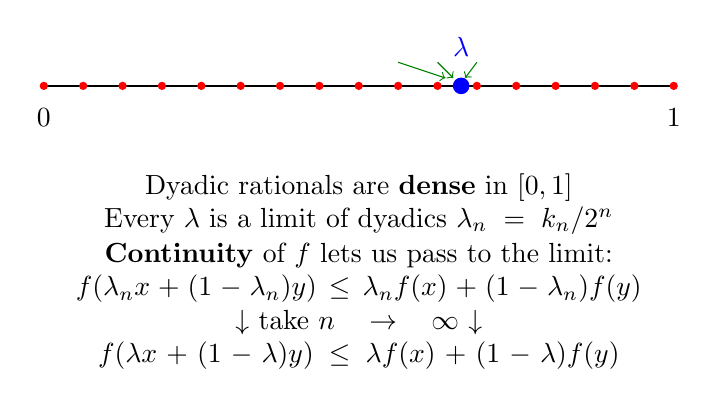
\begin{tikzpicture}[scale=1]
    % Number line [0,1]
    \draw[thick] (0, 0) -- (8, 0);
    \node at (0, -0.4) {$0$};
    \node at (8, -0.4) {$1$};

    % Dyadic rationals (dense!)
    \foreach \k in {0,1,...,16} {
        \pgfmathsetmacro{\x}{\k/2}
        \fill[red] (\x, 0) circle (1.5pt);
    }

    % A general lambda
    \fill[blue] (5.3, 0) circle (3pt);
    \node[blue] at (5.3, 0.5) {$\lambda$};

    % Approximating dyadics
    \draw[green!50!black, ->] (4.5, 0.3) -- (5.1, 0.1);
    \draw[green!50!black, ->] (5.5, 0.3) -- (5.35, 0.1);
    \draw[green!50!black, ->] (5, 0.3) -- (5.2, 0.1);

    \node[text width=8cm, align=center] at (4, -1.5) {Dyadic rationals are \textbf{dense} in $[0, 1]$\\Every $\lambda$ is a limit of dyadics $\lambda_n = k_n/2^n$};
    \node[text width=8cm, align=center] at (4, -2.8) {\textbf{Continuity} of $f$ lets us pass to the limit:\\
    $f(\lambda_n x + (1 - \lambda_n)y) \leq \lambda_n f(x) + (1 - \lambda_n)f(y)$\\
    $\downarrow$ take $n \to \infty$ $\downarrow$\\
    $f(\lambda x + (1 - \lambda)y) \leq \lambda f(x) + (1 - \lambda)f(y)$};
\end{tikzpicture}
\end{center}

\section{Why Continuity is Essential}

Without continuity, midpoint convexity does \textbf{not} imply convexity!

\begin{center}
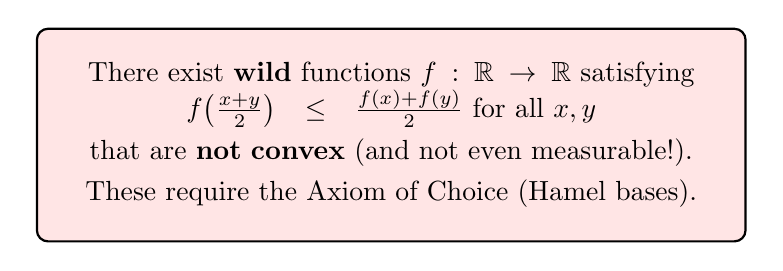
\begin{tikzpicture}[scale=0.9]
    \draw[thick, rounded corners, fill=red!10] (-5, -1.5) rectangle (5, 1.5);
    \node[text width=9cm, align=center] at (0, 0) {
        There exist \textbf{wild} functions $f: \R \to \R$ satisfying\\
        $f\!\left(\frac{x+y}{2}\right) \leq \frac{f(x)+f(y)}{2}$ for all $x, y$\\[0.3em]
        that are \textbf{not convex} (and not even measurable!).\\[0.3em]
        These require the Axiom of Choice (Hamel bases).
    };
\end{tikzpicture}
\end{center}

Continuity is the ``glue'' that forces the midpoint condition to propagate to all $\lambda$.

\section{Contrast with Exercise 23}

\begin{center}
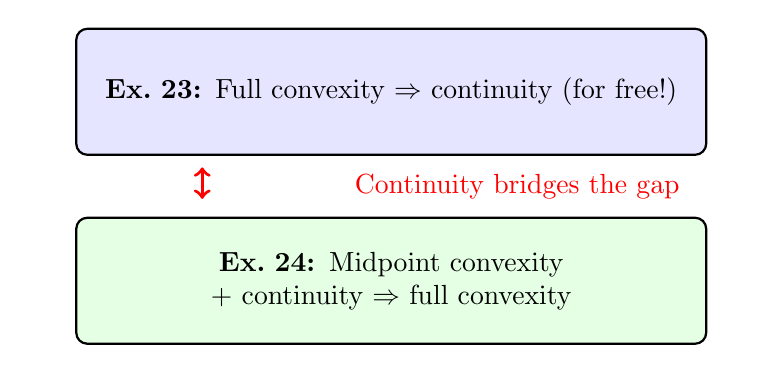
\begin{tikzpicture}[scale=0.8]
    % Ex 23
    \draw[thick, rounded corners, fill=blue!10] (-5, 1) rectangle (5, 3);
    \node[text width=9cm, align=center] at (0, 2) {
        \textbf{Ex.\ 23:} Full convexity $\Rightarrow$ continuity (for free!)
    };

    % Ex 24
    \draw[thick, rounded corners, fill=green!10] (-5, -2) rectangle (5, 0);
    \node[text width=9cm, align=center] at (0, -1) {
        \textbf{Ex.\ 24:} Midpoint convexity + continuity $\Rightarrow$ full convexity
    };

    % Arrow
    \draw[<->, very thick, red] (-3, 0.3) -- (-3, 0.8);
    \node[red] at (2, 0.5) {Continuity bridges the gap};
\end{tikzpicture}
\end{center}

\section{Proof Outline}

\begin{center}
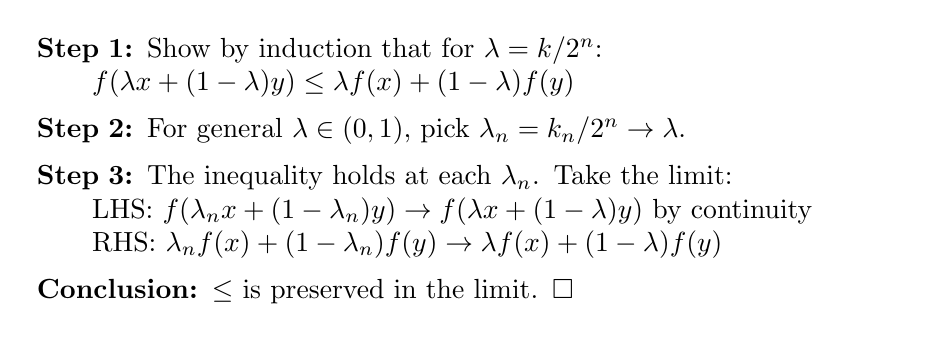
\begin{tikzpicture}[scale=1]
    \node[text width=11cm, align=left] at (0, 0) {
        \textbf{Step 1:} Show by induction that for $\lambda = k/2^n$:\\
        \hspace{2em}$f(\lambda x + (1-\lambda)y) \leq \lambda f(x) + (1-\lambda)f(y)$\\[0.5em]
        \textbf{Step 2:} For general $\lambda \in (0,1)$, pick $\lambda_n = k_n/2^n \to \lambda$.\\[0.5em]
        \textbf{Step 3:} The inequality holds at each $\lambda_n$. Take the limit:\\
        \hspace{2em}LHS: $f(\lambda_n x + (1-\lambda_n)y) \to f(\lambda x + (1-\lambda)y)$ by continuity\\
        \hspace{2em}RHS: $\lambda_n f(x) + (1-\lambda_n)f(y) \to \lambda f(x) + (1-\lambda)f(y)$\\[0.5em]
        \textbf{Conclusion:} $\leq$ is preserved in the limit. $\square$
    };
\end{tikzpicture}
\end{center}

\end{document}
